%%% PREAMBLE - Do not touch %%%%%%%%%%%%%%%%%%%%%%%%%%%%%%%%%%%%%%%%%%%%%%%%%%%%%%
\documentclass[10pt,twocolumn,letterpaper]{article}
\usepackage[ansinew]{inputenc}
\usepackage[portuges,brazil,english]{babel}
\usepackage{model}
\usepackage{times}
\usepackage{epsfig}
\usepackage{graphicx}
\usepackage{amsmath}
\usepackage{amssymb}
\usepackage{color}
\usepackage{float}
\usepackage[pagebackref=true,breaklinks=true,letterpaper=true,colorlinks,bookmarks=false]{hyperref}

\cvprfinalcopy % *** Uncomment this line for the final submission
\def\httilde{\mbox{\tt\raisebox{-.5ex}{\symbol{126}}}}
\ifcvprfinal\pagestyle{empty}\fi

\newcommand{\TODO}[1]{TODO: #1}
\newcommand{\CITEONE}[2]{\mbox{#1 \cite{#2}}}
\newcommand{\CITETWO}[3]{\mbox{#1 and #2 \cite{#3}}}
\newcommand{\CITEN}[2]{\mbox{#1 et al. \cite{#2}}}

%%% Paper beginning %%%%%%%%%%%%%%%%%%%%%%%%%%%%%%%%%%%%%%%%%%%%%%%%%%%%%%%%%%%%%%
\begin{document}

%%% Title and authors %%%%%%%%%%%%%%%%%%%%%%%%%%%%%%%%%%%%%%%%%%%%%%%%%%%%%%%%%%%%
\title{Assignment 3 - MO444}
\author{Pedro Henrique M. X. Zacarin\thanks{\textbf{Contact}: \tt\small{phzacarin@gmail.com}}\\
}

%%% Abstract %%%%%%%%%%%%%%%%%%%%%%%%%%%%%%%%%%%%%%%%%%%%%%%%%%%%%%%%%%%%%%%%%%%%%
\maketitle
\begin{abstract}
In this assignment, the goal was to clusterize all the headlines from a dataset consisting of 1 million headlines from the Australian Broadcast Corporation (ABC) over a period of 15 years based on topics.
\end{abstract}

%%% Introduction %%%%%%%%%%%%%%%%%%%%%%%%%%%%%%%%%%%%%%%%%%%%%%%%%%%%%%%%%%%%%%%%%
\section{Introduction}
Thousands of headlines are generated every day from news sources around the world. Normally, those headlines are categorized inside its source, such as newspapers, magazines and websites.

The categorization and clustering of a set of news is something very useful in various fields: search engines so it can find results based on a given topic, news aggregators that uses web crawlers to find content so it can filter through topics and recommendation systems that can offer news similar to the ones that are being read, or to the reader's content.

In this assignment, a dataset consisting of 1 million headlines from the Australian Broadcast Corporation (ABC) was given, so the headlines could be clusterized in topics utilizing unsupervised learning methods such as KMeans.

%%% Add section %%%%%%%%%%%%%%%%%%%%%%%%%%%%%%%%%%%%%%%%%%%%%%%%%%%%%%%%%%%%%%%%%%
\section{Feature extraction}
To solve the given problem, a set of features needs to be extracted from the headlines.

To gather the needed features, the first step was to clean every headline to make it suitable for a bag-of-words representation. To do so, the following steps were taken:
\begin{itemize}
	\item All numbers were removed
	\item All stop-words (like connection words that are not relevant to classification) were removed
	\item All words in each headline was replaced with its stem word (word without prefixes or suffixes) 
\end{itemize}

After all headlines were cleaned, n-grams were extracted from all of them. For this assignment, char-4-grams was chosen because in other experiments [REFERENCIA ANDERSON] the result achieved was better than word-level n-grams. By choosing char-4-grams, it means that the n-grams extracted were consisted of 4 chars, including spaces, from the original headline.

Once all char-4-grams were extracted, they were sorted by occurrence frequency and only about the top 15$\%$ in the ranking were considered in the feature extraction process. A relatively small amount of the most frequent n-grams were considered because its total number together with the total number of headlines to be analyzed is too big, which caused many problems regarding exceeding memory consumption and Python environment kernel deaths.

With the most frequent char-4-grams in hand, the feature matrix was build following the steps below:
\begin{enumerate}
	\item Build a hash of the most frequent char-4-grams as keys and its occurrences frequencies as values
	\item Create a zero-filled matrix with the number of rows being the number of total headlines and the number of columns being the total number of char-4-grams in the previous step's hash
	\item For each char-4-gram (or, for each column $j$ in the matrix), count its frequency in each headline (each row $i$ of the matrix) and assign this number to the associated position $(i,j)$ in the feature matrix. This calculation is called $tf$, which means $therm frequency$.
	\item Calculate, for all char-4-grams, its $idf$ ($inverse document frequency$) and create a diagonal matrix with those values
	\item Calculate the $tf*idf$ matrix by multiplying both $tf$ and $idf$ matrices
	\item Apply L2 normalization to the final matrix
\end{enumerate}

With all the steps above done, the final feature matrix is complete.

%%% Add section %%%%%%%%%%%%%%%%%%%%%%%%%%%%%%%%%%%%%%%%%%%%%%%%%%%%%%%%%%%%%%%%%%
\section{Clustering}
In order to separate all headlines into groups, K-Means algorithm was chosen. This method aims to partition the dataset so as to minimize the within-cluster sum of squares (or variance).

As the standard K-Means is computationally intensive when using the whole dataset of headlines,  a simpler, faster derivation of it was chosen, with minimal impacts in the final results: mini batch KMeans. In this approach, a small random batch is taken for each iteration and for each data point in this batch a cluster is assigned  depending on the previous locations of the cluster centroids. It then updates the location of cluster centroids based on the new points from the batch. 

\section{Execution and Results}

For the whole dataset of 1 million headlines, mini batch KMeans was run with a batch of $100$, initialization being KMeans++ and K ranging from 2 to 20. The cost (inertia) for each K was plotted in a chart so the optimal number of K could be assessed by the elbow rule.

\begin{figure}[H]
\begin{center}
	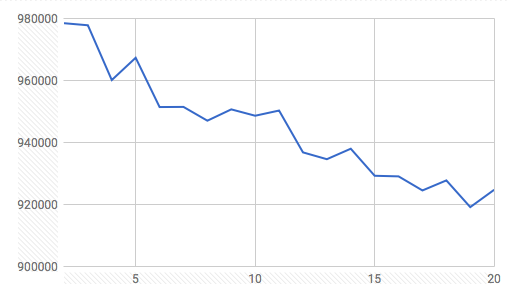
\includegraphics[width=0.4\textwidth]{pics/graph_inertia_all}
	\caption{Cost (inertia) of mini batch KMeans vs value of K\label{fig:graph_inertia_all}}   
\end{center} 
\end{figure}   

Analyzing the Figure ~\ref{fig:graph_inertia_all}, it can be seen that the smallest cost was achieved with K = $19$, so that number was utilized to perform the final clustering process and the analysis of each one's content.

To analyze the results, all headlines assigned to each cluster were separated in lists. From those headlines, its word-level 1-grams were extracted and put in order of occurrences, so the key words for each cluster could be easily assessed and consequently, the cluster's topic found.



%%% Add section %%%%%%%%%%%%%%%%%%%%%%%%%%%%%%%%%%%%%%%%%%%%%%%%%%%%%%%%%%%%%%%%%%
\section{Discussion}
%%%Talk about the experiments carried out and the obtained results. 

\CITEONE{Silva}{Silva_2010} for papers with one author.
\CITETWO{Silva}{Souza}{Silva_2010b} for papers with two authors.
\CITEN{Silva}{Silva_2010c} for papers with three or more authors.

The standard model for linear regression, when run with a gradient descent algorithm for optimizing the values of theta and with all its features normalized, resulted in a considerably high average error of 3000 shares for the training set and 3177 shares for the test set.

Some modifications were applied to the standard linear regression model in order to find better values of thetas that minimized the cost function. As the features in the training set were taken to higher powers (up to 12th) and added to it, a very small drop in the training set average error (0.4$\%$) was obtained, together with a slight increase in the test set average error (0.9$\%$), showing a glimpse of overfitting. In order to try to mitigate the effects of overfitting, regularization was used, and, with a $\lambda$ = 100000, the difference between the training and test average errors was reduced (3020 and 3190 shares, respectively), but the net error suffered an increase.

When only the continuous features were used, the errors obtained from the training set increased by 0.7$\%$ compared to the initial method and the ones from the test set increased by 0.6$\%$, a very small amount.

By utilizing the normal equations method, which gives an optimal value for the thetas utilizing a pure linearization model, a resulting average training set error of 2999 shares, almost the same as the result found initially (3000 shares) was found.

%%% Add section %%%%%%%%%%%%%%%%%%%%%%%%%%%%%%%%%%%%%%%%%%%%%%%%%%%%%%%%%%%%%%%%%%
\section{Conclusions}

After utilizing various methods and improvements based on linear regression in order to improve the error in the prediction of number of shares, none of them resulted in an acceptable error. 

The minimum average error was 2999 shares for the training set and 3177 shares for the test set utilizing normal equations. A better number was found adding higher order features to the training set (2987 shares), but the distance between its error and the test set one (3204 shares) was higher (overfit). Moreover, trying to reduce the effects of overfitting by using regularization also didn't lead to a better result.

The conclusion that can be taken from the approaches taken is that linear regression is not a good model to represent the problem, and a more complex model must be used in order to account for all the non linearities and intricacies of the dataset.

%%% References %%%%%%%%%%%%%%%%%%%%%%%%%%%%%%%%%%%%%%%%%%%%%%%%%%%%%%%%%%%%%%%%%%%
{\small
\bibliographystyle{unsrt}
\bibliography{referencias-exemplo}
}

\end{document}